\subsection{几乎处处有定义的函数}

按照 No.~3 中的定义，从 X 的子集 A 到集合 F 中的映射 f 称为几乎处处有定义的，如果它在其上定义的集 A 的余集是可忽略集。我们仍称 f 的等价类（记作 \(\widetilde{f}\) ）为下述每个函数的等价类：该函数定义在整个 X 上，且在 f 有定义的点处等于 \(f(x)\) （诸点 \(x \in X\) ）；显然这个类只依赖于 f。~两个几乎处处有定义的函数 f, g 当 \(\widetilde{f} = \widetilde{g}\) 时仍称为等价的：这就是说，使 \(f(x)\) 与 \(g(x)\) 都有定义且相等的点所成的集具有可忽略的余集。

由此立即推出，No.~4 的命题 8 及其推论可以推广到下述情形：在其叙述中只假设每个函数 \(f_{n}, g_{n}\) 都几乎处处有定义；这时函数 \(\varphi((f_{n}))\)

和 \(\varphi((g_n))\) 本身也几乎处处有定义；\(\varphi((f_n))\) 的等价类仍是 \(\varphi((\widetilde{f}_n))\) 。

一个几乎处处有定义、取值于向量空间 F 中的函数，如果等价于 0，仍称为可忽略的。若 f 是取值于 F 中的可忽略函数，而 u 是从 F 到向量空间 G 中的线性映射，则复合函数 \(u \circ f\) （几乎处处有定义）是可忽略的；类似地，对每个几乎处处有定义的（有限）数值函数 g，函数 gf （几乎处处有定义）是可忽略的。

\pandocbounded{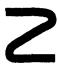
\includegraphics[keepaspectratio]{images/part001_e94daaaa.jpg}}

必须注意，在取值于 F 且几乎处处有定义的函数所成的集中，内合成法则 \((\mathbf{f},\mathbf{g})\mapsto\mathbf{f}+\mathbf{g}\) 不是群法则，因为虽然函数 0 确是此法则的中性元，但若 f 不是处处有定义，则不存在使 \(f+g=0\) 的函数 g。这正是引入等价类 \(\widetilde{f}\) 的动机，这些类确实构成一个向量空间。

设 \((f_n)\) 是映射到拓扑空间 F 中的一列映射，其中每个都在 X 中几乎处处有定义。我们说序列 \((f_n)\) 在 X 中几乎处处（逐点）收敛于 f，如果由下述点 \(x \in X\) 组成的集具有可忽略的余集：所有 \(f_n(x)\) 在该点有定义，且序列 \((f_n(x))\) 有等于 \(f(x)\) 的极限。显然，若对每个 n，函数 \(g_n\) （几乎处处有定义）等价于 \(f_n\) ，则序列 \((g_n)\) 也几乎处处收敛于 f。

若 F 是拓扑向量空间，则类似地定义一个几乎处处收敛的级数，其通项是在 X 中几乎处处有定义、取值于 F 中的函数 \(f_{n}\) ；这个级数的和是在部分和 \(\sum_{k=1}^{n}\mathbf{f}_{k}(x)\) 有定义且有极限的那些点处有定义的函数，其类只依赖于诸类 \(\widetilde{f}_{n}\) 。

